\documentclass[border=10pt]{standalone}

\usepackage{tikz}
\usepackage{tikzsymbols}
\usetikzlibrary{calc,patterns,shapes.geometric}

\def\centerarc[#1](#2)(#3:#4:#5){\draw[#1] ($(#2)+({#5*cos(#3)},{#5*sin(#3)})$) arc (#3:#4:#5);}

\begin{document}
	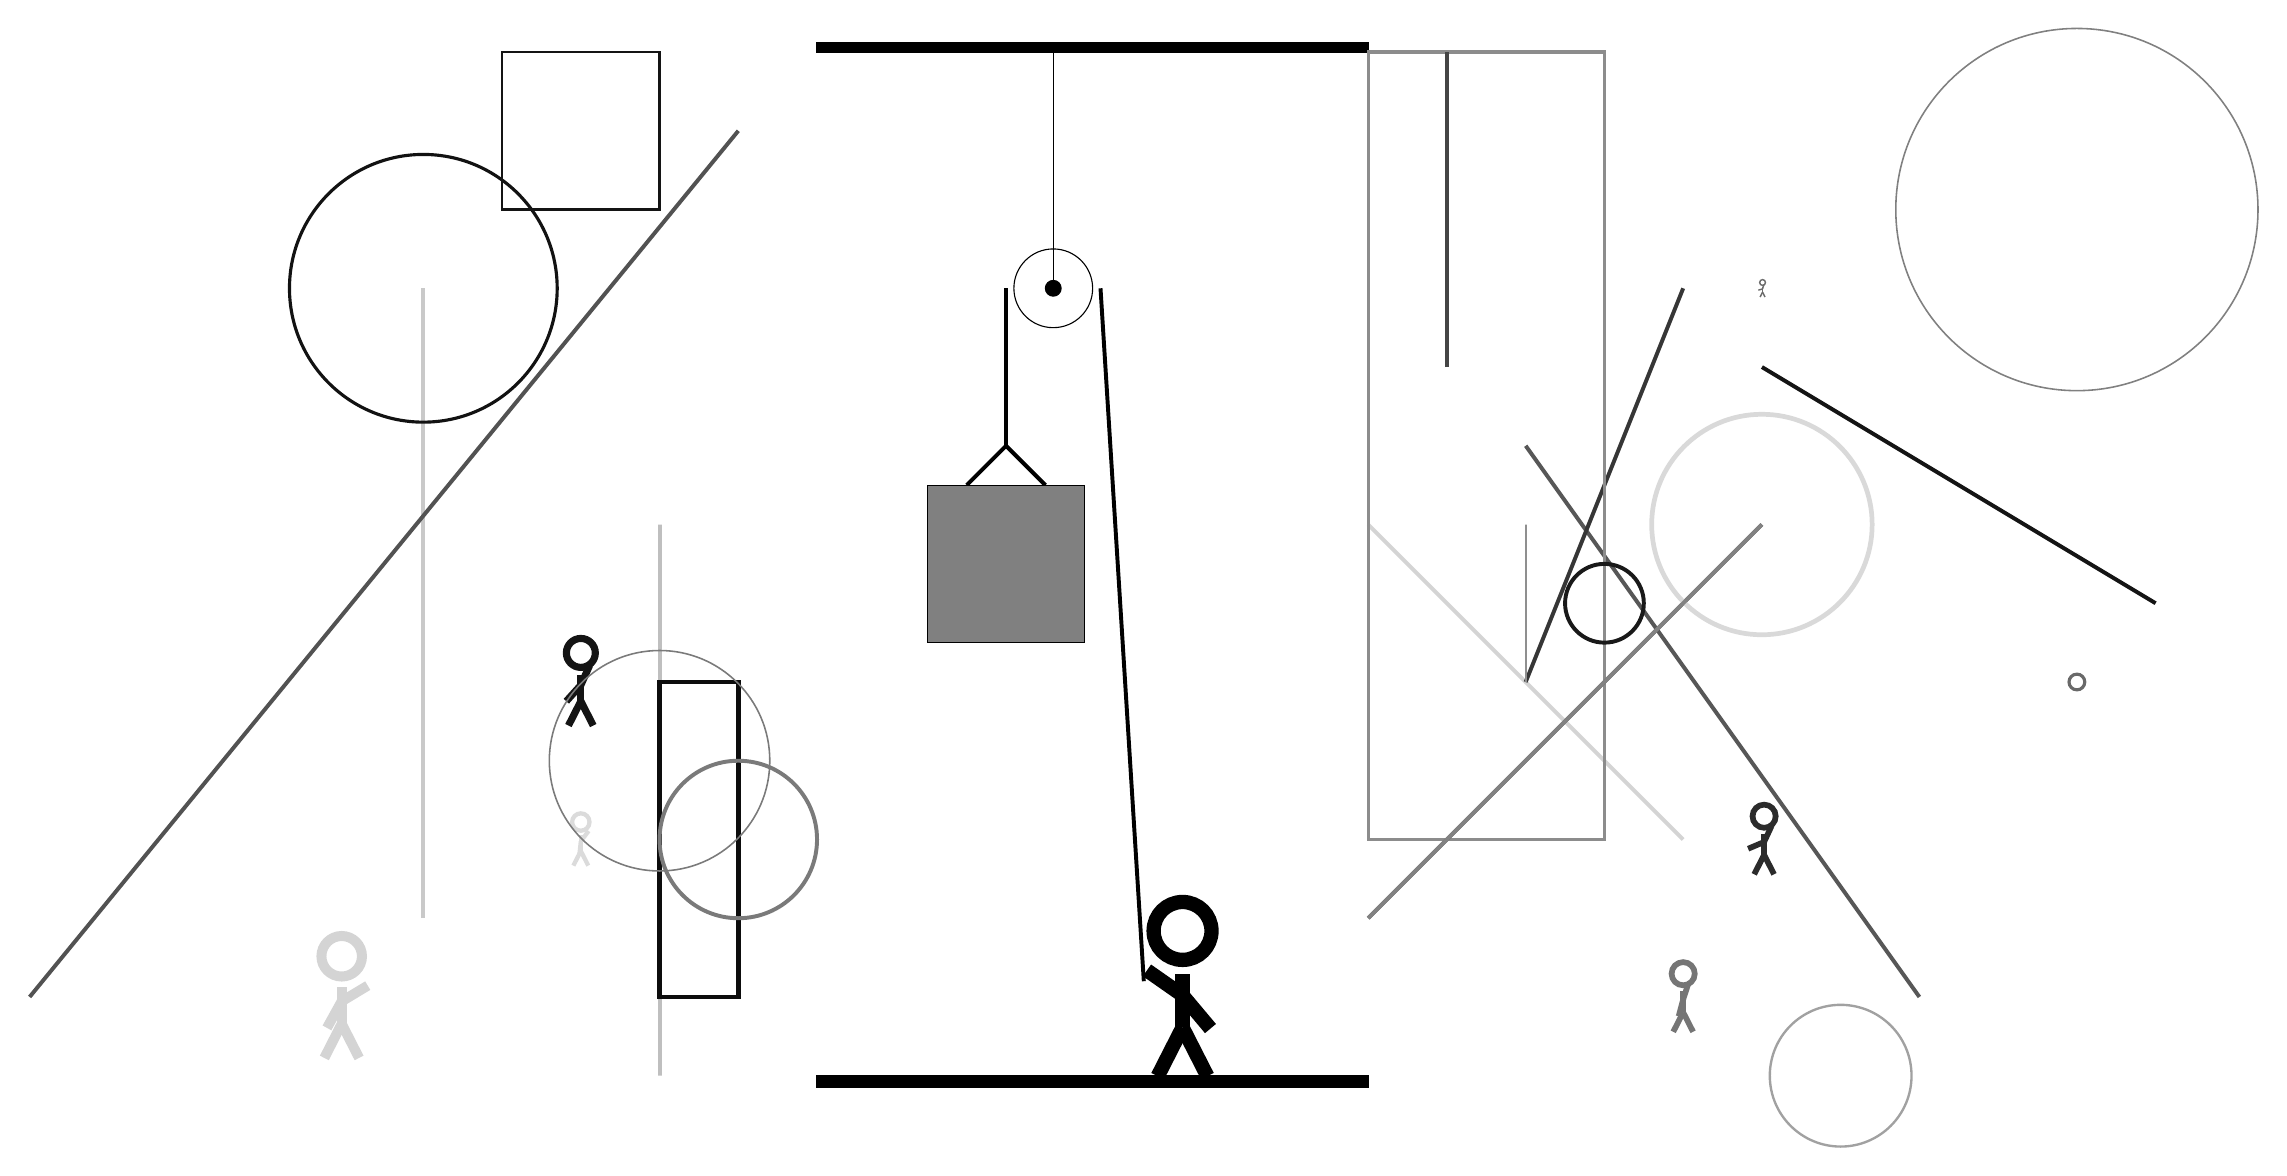
\begin{tikzpicture}
		%%%%% START %%%%%
		
		\draw[fill=black] (-2, 10) rectangle (5, 10.125);
		
		\draw (1, 7) circle (0.5);
		\draw[fill=black] (1, 7) circle (0.1);
		\draw (1, 10) -- (1, 7);
		
		\draw[line width=0.5mm] (-0.1, 4.5) -- (0.4, 5.0) -- (0.9, 4.5);
		\draw[fill=black!50] (-0.6, 4.5) rectangle (1.4, 2.5);
		
		\draw[line width=0.5mm] (0.4, 7) -- (0.4, 5.0);
		\centerarc[line width=0.5mm](1, 7)(0:180:0.6);
		\draw[line width=0.5mm](1.6, 7) -- (2.15, -1.8);
		
		\node at (2.6, -1.9) {\Strichmaxerl[10][-35][-50]};
		
		\draw[line width=0.5mm, color=black!92](10, 6) -- (15, 3);
		
		\draw[line width=0.5mm, color=black!25] (-4, -3) rectangle (-4, 4);
		\draw[line width=0.6mm, color=black!95] (-4, -2) rectangle (-3, 2);
		\draw [line width=0.5mm, color=black!10](-11, 1) circle (0.0);
		
		\draw[line width=0.5mm, color=black!21](-7, -1) -- (-7, 7);
		
		\draw [line width=0.4mm, color=black!93](-7, 7) circle (1.7);
		\draw[line width=0.5mm, color=black!66](7, 5) -- (12, -2);
		\draw[line width=0.5mm, color=black!17](9, 0) -- (5, 4);
		\draw[line width=0.5mm, color=black!79](7, 2) -- (9, 7);
		
		\draw[line width=0.5mm, color=black!68](-3, 9) -- (-12, -2);
		
		\node[line width=0.4mm, color=black!14] at (-5, 0) {\Strichmaxerl[3][84][53]};
		\draw[line width=0.4mm, color=black!45] (5, 10) rectangle (8, 0);
		\draw[line width=0.2mm, color=black!44] (7, 2) rectangle (7, 4);
		
		\draw [line width=0.3mm, color=black!37](11, -3) circle (0.9);
		\draw [line width=0.4mm, color=black!59](14, 2) circle (0.1);
		\draw [line width=0.2mm, color=black!50](14, 8) circle (2.3);
		\node[line width=0.6mm, color=black!92] at (-5, 2) {\Strichmaxerl[5][48][66]};
		\draw[line width=0.5mm, color=black!63](10, 4) -- (5, -1);
		\draw [line width=0.5mm, color=black!90](8, 3) circle (0.5);
		
		\draw [line width=0.2mm, color=black!52](-4, 1) circle (1.4);
		\node[line width=0.3mm, color=black!54] at (9, -2) {\Strichmaxerl[4][75][72]};
		\draw[line width=0.5mm, color=black!73](6, 6) -- (6, 10);
		\draw [line width=0.6mm, color=black!15](10, 4) circle (1.4);
		\node[line width=0.4mm, color=black!58] at (10, 7) {\Strichmaxerl[1][16][73]};
		\draw[line width=0.3mm, color=black!92] (-4, 8) rectangle (-6, 10);
		\draw[line width=0.5mm, color=black!49](10, 4) -- (5, -1);
		\draw [line width=0.5mm, color=black!52](-3, 0) circle (1.0);
		\node[line width=0.5mm, color=black!17] at (-8, -2) {\Strichmaxerl[7][61][31]};
		
		\draw [line width=0.3mm, color=black!34](10, 8) circle (0.0);
		\node[line width=0.6mm, color=black!83] at (10, 0) {\Strichmaxerl[4][23][65]};
		
		\draw[fill=black] (-2, -3) rectangle (5, -3.15);
		
		%%%%% END %%%%%
	\end{tikzpicture}
\end{document}